\documentclass[mla8]{mla}

\title{Sample MLA Document}
\author{John Doe}
\professor{Dr. Suzie Que}
\course{\LaTeX\ 101}
\date{\mladate} % see docs for `\mladate'

% The .bib file (explained later) must be included in the preamble
\addbibresource{mla-example.bib}

\begin{document}

\begin{paper}

This is an example document using ``mla.cls''.
The header is automatically printed upon using the ``paper'' class,
which is why there is no ``\textbackslash{}maketitle''.

\section{Professors who prefer sections}

Sometimes, research papers can become unmanageably lengthy.
In that case, section headings can help divide up the ideas
to make it more accessible to the reader.
Though this paper is short, section headings are employed
as an example of the ``mla'' class' capabilities.

Some professors may explicitly require or denounce use of headings.
Dr. Suzie Que of Anytown, PA requires they be used for anything
longer than five pages:
\begin{blockquote}
John---so help me God---if you turn in another twenty-page research
paper with no logical breaks I will hang you at the stake.
Even though the MLA style guide doesn't say anything about
section headings, they're not actually prohibited.
So, if you turn in \emph{anything} longer than five pages to me
and there isn't a \emph{single} break or section heading,
I will dock your grade to an F.
Capisce? \cite{que2019}
\end{blockquote}
Despite her language, she does have a point to say.

\subsection{Subsections}

Alongside regular top-level sections, one can use
``\textbackslash{}subsection'' commands too\endnote{Section commands
in ``mla.cls'' work identical to those of the ``article'' class.}.

\section{Lists}

Vertical lists are a rarity in MLA format, but if one so pleases,
they can be used.
The ``itemize'', ``enumerate'' and ``description'' lists
work just as expected, even with sublists.

\begin{itemize}
\item A bogus item
\item Lorem ipsum dolor sit amet.  This item has a bunch of text
	just so it covers more than one line in the paper and shows
	proper indentation.
\item Last item!
\begin{enumerate}
\item Just kidding; there's a subitem.  And it's a number!
\end{enumerate}
\item Okay, now it's the last item.
\end{itemize}

\section{Figures}

On rare occasions, you might have to use figures or tables
in your paper.
Good news is the ``figure'' and ``table'' environments
work exactly as expected!
Just make sure to use ``\textbackslash{}begin\{figure\}[H]''
if you want the image to stay exactly where you put it.
\begin{figure}[H]
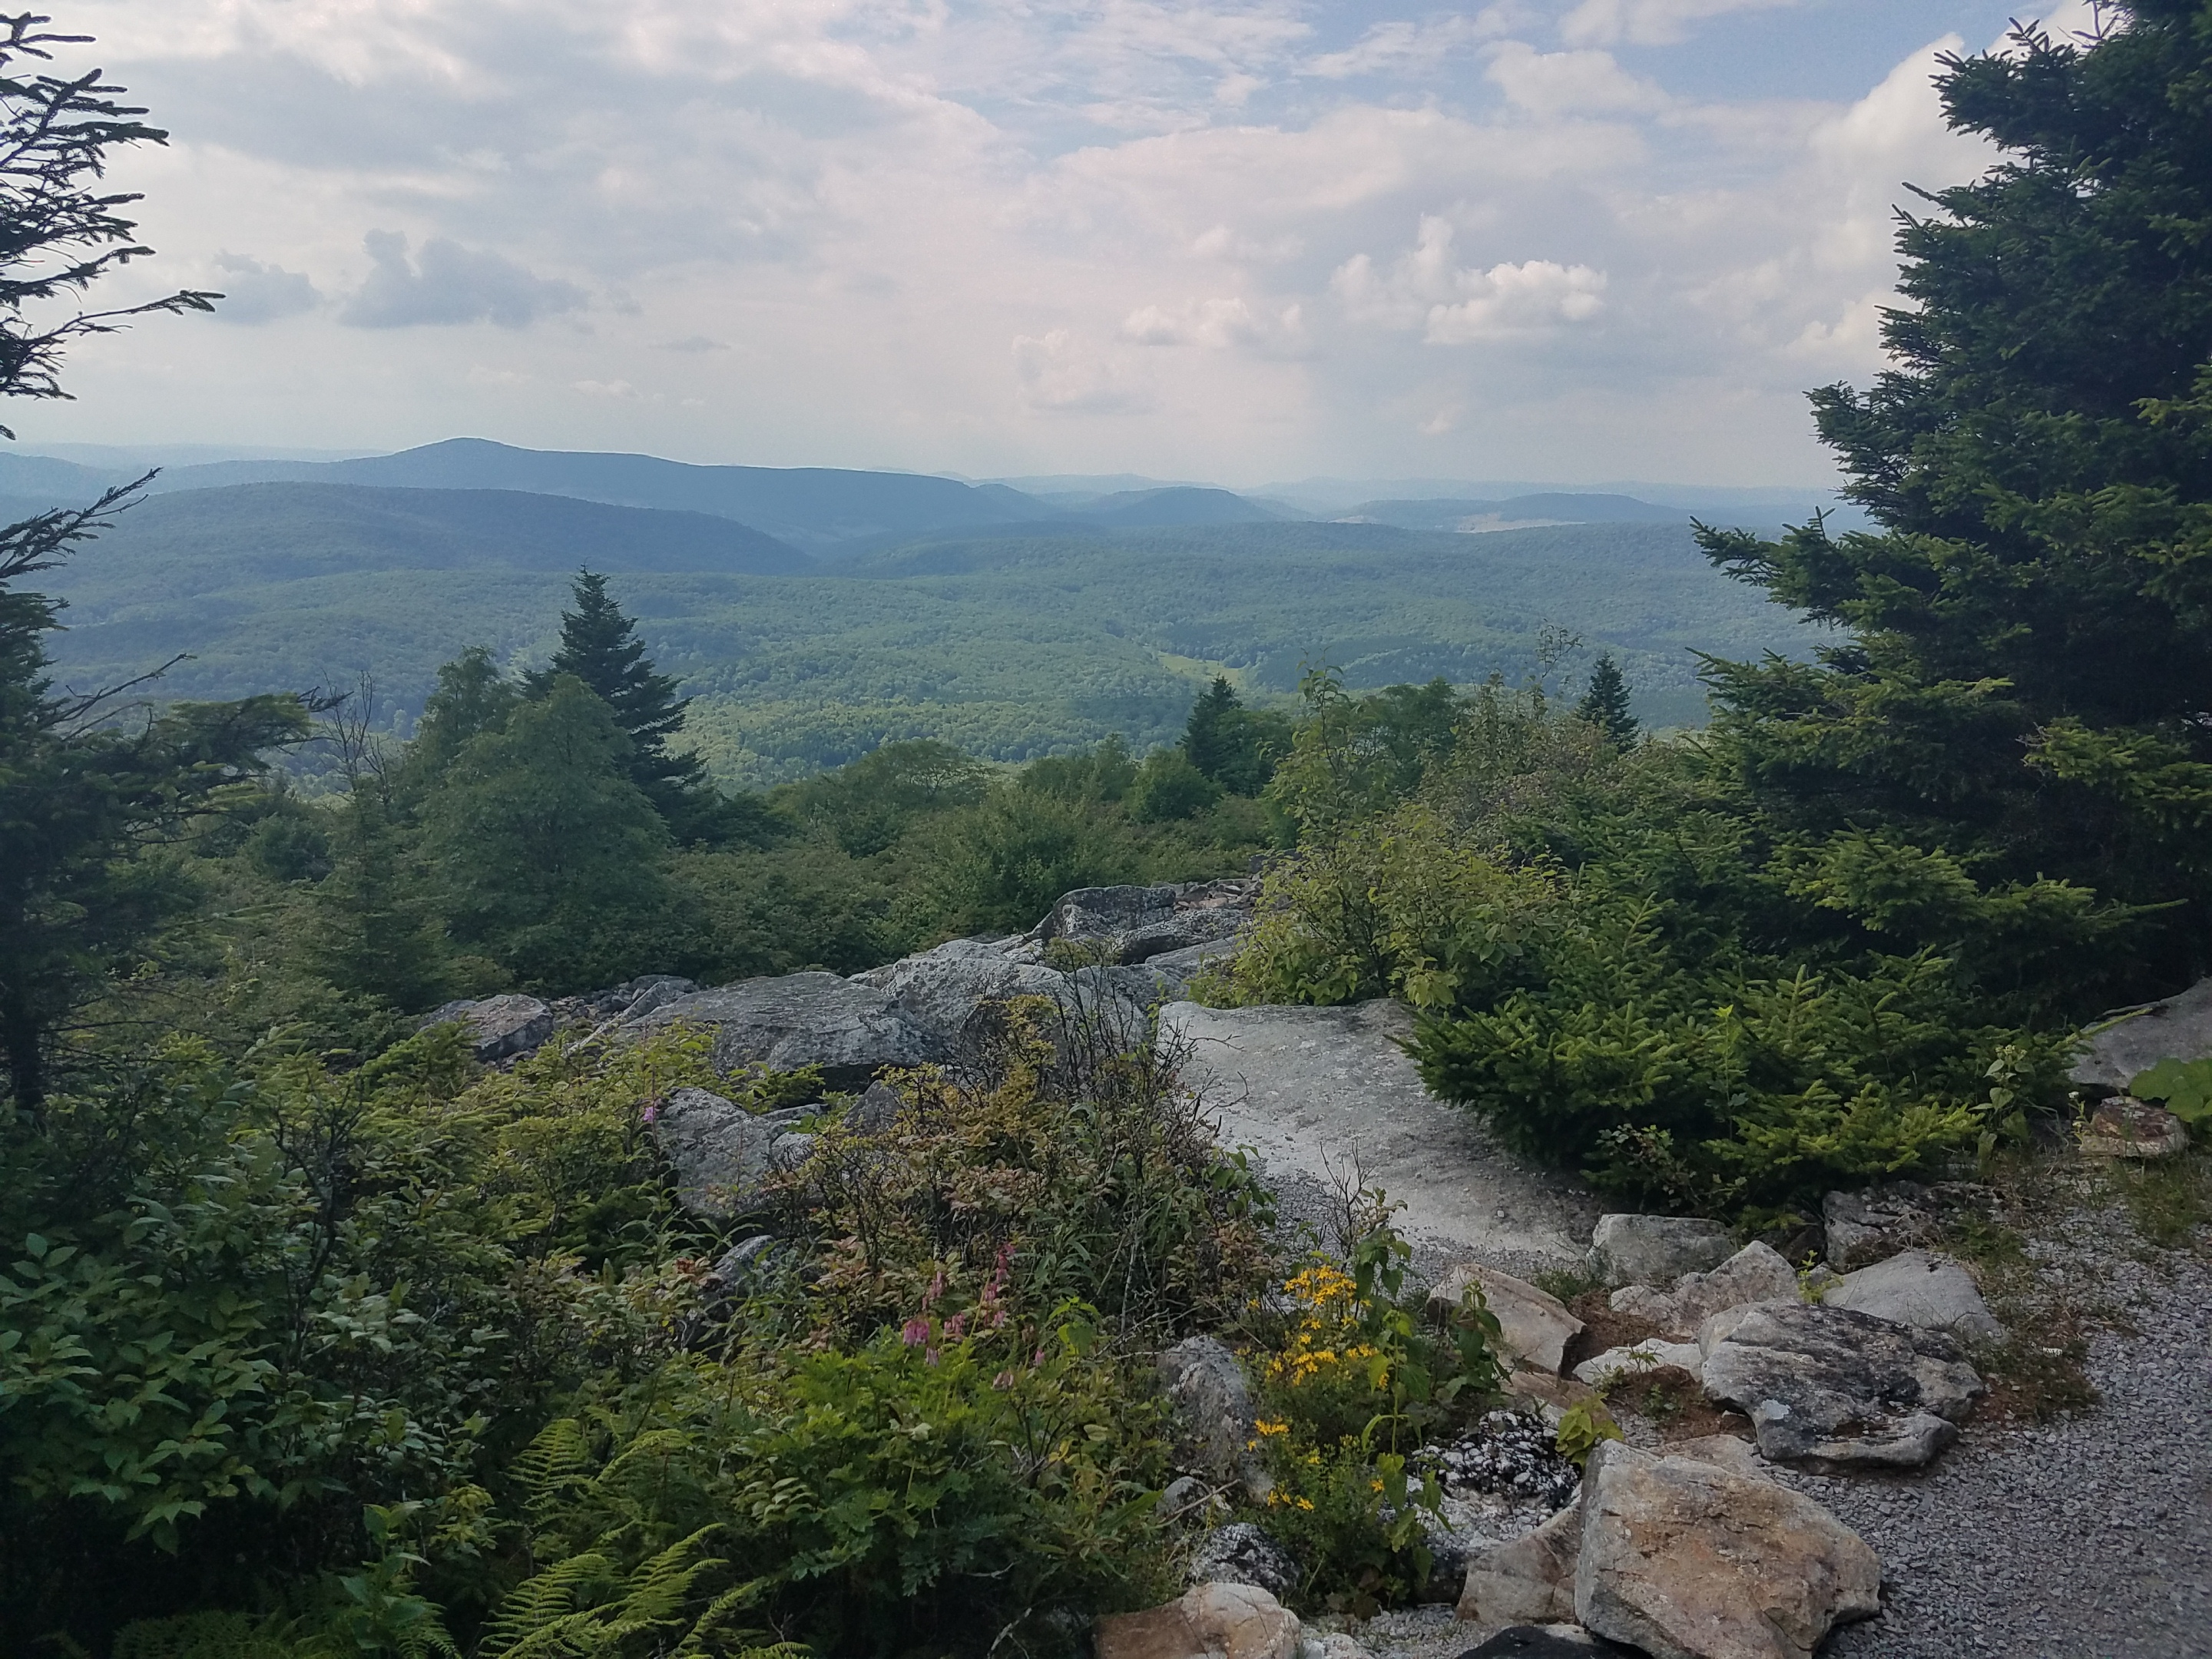
\includegraphics[width=0.5\linewidth]{mla-example-image}
\caption{A scene from atop Spruce Knob, West Virginia}
\end{figure}
And yes, I shamelessly used my own image.

\section{Using endnotes}

As one may notice, the above subsection used an endnote.
These can simply be cited with
``Yada yada text\textbackslash{}endnote\{more info\ldots\}.''
Endnotes can be easily printed in correct format by calling
``\textbackslash{}printendnotes'' within the
``notes'' environment.

\section{Using bibliographies}

Dr. Suzie Que was cited in the above blockquote.
The ins-and-outs of ``biblatex'' will not be explained in this
document, so please refer to online documentation such as the
``BibLaTeX Cheat Sheet''.

Just as with the endnotes,
the bibliography can be easily printed in correct format by calling
``\textbackslash{}printbibliography[heading=none]'' within the
``workscited'' environment.
(The ``heading=none'' part is important; the ``workscited'' environment
already prints one.)

\end{paper}

\begin{notes}

\printendnotes

\end{notes}

\begin{workscited}

\printbibliography[heading=none]

\end{workscited}

\end{document}
